\section{Desugaring}
\label{sec:desugar}


The section provides the procedures of desugaring traits to \bname. The idea
behind trait translation is inspired by the functional mixin semantics using
open recursion, which is proposed by~\citet{cook1989denotational} in an untyped
setting. However, our translation is done in the context of a statically-typed
programming language, which is exactly why conflicts can be \textit{statically}
detected in traits.

\subsection{Trait Declarations}

Essentially traits are translated into term declarations, with methods becoming
record fields. The self-reference is adjusted to be the last parameter of the
declaration. For example,
\begin{lstlisting}
  trait point(x : Int, y: Int) { self : Point =>
    def x() = x
    def y() = self.x()
  }
\end{lstlisting}
becomes
\begin{lstlisting}
  def point (x : Int) (y : Int) (self : Point) =
  { x = \_ -> x
  , y = \_ -> self.x()
  }
\end{lstlisting}

Now it is clear that \lstinline{self} is not a special keyword: it can
have any name.

More formally, a trait of the form
\begin{lstlisting}[mathescape=true]
  trait m [$A_1$, ..., $A_n$] ($x_1 : A_1$, ..., $x_n : A_n$) inherits $a_1$ & ... & $a_n$ { s : $A_0$ =>
    def $m_1$(...) = $e_1$
    ...
    def $m_n$(...) = $e_n$
  }
\end{lstlisting}
is translated into a term declaration of the form
\begin{lstlisting}[mathescape=true]
  def m $A_1$ ... $A_n$ $(x_1 : A_1)$ ... $(x_n : A_n)$ $(s : A_0)$ = $a_1$(s) ,, ... ,, $a_n$(s) ,,
  {
    $m_1$ = \(...) -> $e_1$
  , ...
  , $m_n$ = \(...) -> $e_n$
  }
\end{lstlisting}


\subsection{Instantiations of Traits}

\name allows creating a single object from one or more traits. Specifically,
\lstinline{new} instantiates a trait by taking the fixpoint of its
corresponding open term. In fact, \lstinline{new} is translated as an inlined
fixpoint. For example,
\begin{lstlisting}
  new[Point] point(3,4)
\end{lstlisting}
becomes
\begin{lstlisting}
  let self : Point = point 3 4 self in self
\end{lstlisting}
Essentially the open term is closed using \textit{lazy fixpoints}. Lazy
fixpoints are a standard way to encode dynamic mixin inheritance and bind
self-reference in denotational semantics~\cite{cook1989denotational}.

Lazy fixpoints are implemented in \name using the built-in \lstinline{let}
construct (possibly recursive), which employs call-by-name semantics. It is
possible to choose call-by-value, then the type of the self-reference would
becomes a thunk, that is, \lstinline$T -> Point$.

The composition of traits in the \lstinline{new} expression is desugared using
the merge operator. Now it is clear that the reason traits have conflict
detection for free is that the merge operator is enforcing two terms being
merged are disjoint. For example,
\begin{lstlisting}
  new[Point & Norm] point(3,4) & euclideanNorm()
\end{lstlisting}
is turned into
\begin{lstlisting}
  let self : Point & Norm = (point 3 4 self) ,, (euclideanNorm () self) in self
\end{lstlisting}

Formally, a \lstinline{new} expression of the form
\begin{lstlisting}[mathescape=true]
  new[$A_1$ & ... & $A_n$] $a_1$ & ... & $a_n$
\end{lstlisting}
is translated into a let expression of the form
\begin{lstlisting}[mathescape=true]
  let self : $A_1$ & ... & $A_n$ = $a_1$(self) ,, ... ,, $a_n$(self) in self
\end{lstlisting}

\subsection{The Type for Traits}

\lstinline[mathescape=true]{Trait[$T_1, T_2$]} denotes the type of those traits
which provide an interface described by the type $T_2$ with dependency on $T_1$.
In fact, it is just like a type constructor except for the fact that it is
built-in in the language, and that the encoding is not exposed to the
programmers.

Formally, a trait type of the form \lstinline[mathescape=true]{Trait[$T_1, T_2$]} becomes \lstinline[mathescape=true]{$T_1$ -> $T_2$}.


\section{Implementation}

The \name prototype implementation is structured around a typed core language
(\bname with some extensions). The main component of the implementation is an
elaborating type-checker, which takes a \bname expression, checks it, and
produces another expression in the target language. The final expression is then
directly executed by an interpreter. We chose call-by-name untyped lambda
calculus as the target language. Since we focus on the implementation, and types
are irrelevant after type checking, untyped lambda calculus is a suitable choice
with minimal syntax. With some simple optimization, the interpreter delivers
reasonably good execution efficiency.

The overall implementation is unremarkable, as it closely follows the semantics
that was presented by~\citet{alpuimdisjoint}. The whole pipeline is shown in
Figure~\ref{fig:pipeline}. The desugaring phase (cf. Section~\ref{sec:desugar})
takes a simple abstract data type (AST) generated by the parser, and returns a
\bname expression. Traits-related constructs disappear after this phase. The
type checking phase then takes a \bname expression from the previous phase, it
infers and checks its type, and in the meantime, produces an expression in the
target language. The type checker is the most involved component in the
pipeline. It contains a (coercive) subtyping procedure and a disjointness
checker, both of which are the most essential parts for \name to work as we
wanted it. The target expression (pure untyped lambda calculus) then enters the
final phase, and is executed by a simple interpreter.

The prototype implementation is written in just 1400 lines of Haskell code.

\begin{figure}
  \centering
  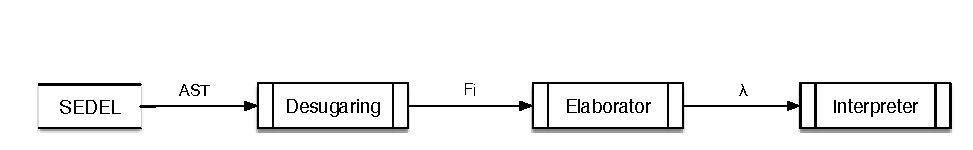
\includegraphics[scale=0.9]{pipeline.eps}
  \caption{The pipeline of \name}
  \label{fig:pipeline}
\end{figure}